\section{WebRTC DataChannel} \label{chapter_datachannel}

Text. Figure \ref{fig:http} Figure \ref{fig:websocket}

\begin{figure}[htp]
  \begin{center}
    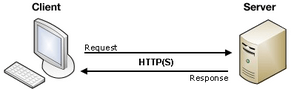
\includegraphics[width=0.9\columnwidth]{resources/http.png}
  \end{center}
  \caption{HTTP communication [developer.mozilla.org]}
  \label{fig:http}
\end{figure}

Text. Figure \ref{fig:webrtc}

\begin{figure}[htp]
  \begin{center}
    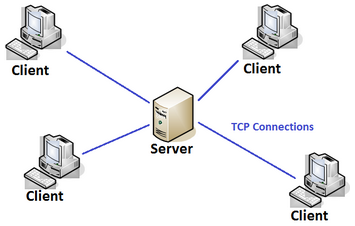
\includegraphics[width=0.9\columnwidth]{resources/websocket.png}
  \end{center}
  \caption{Client-server architecture [cs.montana.edu]}
  \label{fig:websocket}
\end{figure}

\begin{figure}[htp]
  \begin{center}
    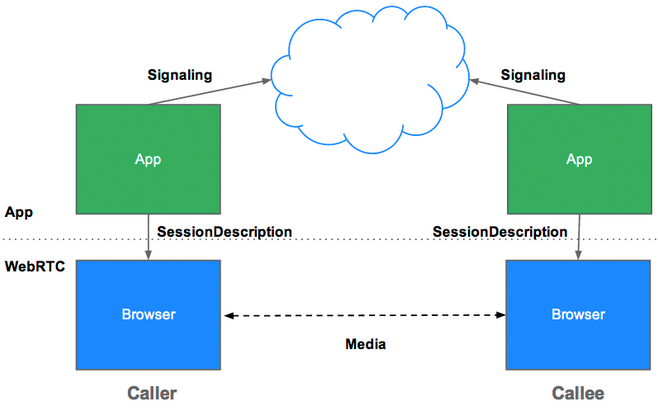
\includegraphics[width=0.9\columnwidth]{resources/webrtc.png}
  \end{center}
  \caption{WebRTC overview [html5rocks.org]}
  \label{fig:webrtc}
\end{figure}

Text.

\subsection{Compatibility}

Text.
